\chapter{Megvalósítás}

A koncepció átbeszélése után áttérhetünk az implementációra. Egy Godot projekt Node-okból tevődik össze, amelyeket egy fa struktúrába rendezve tudunk kezelni. Érdemes egy Node-ra úgy tekinteni, mint egy osztályra, mivel valójában az is. Minden ilyen fát egy ún. "színteren" belül helyezünk el. Ez arra szolgál, hogy egyes részeit a projektünknek külön tudjuk kezelni a többitől, ez majd jobban világossá fog válni, amikor a játékos színteréről beszélek. Egy színtér felépítésében fontos szerepet játszik a Node hierarchia kialakítása. Vannak ugyanis Node-ok, amelyek megkövetelnek más Node-okat, mint gyermeket ahhoz, hogy rendesen működjön. Ilyen például egy StaticBody3D (egy statikus, fizikai erőkkel nem mozgatható test reprezentálá\-sára szolgál a háromdimenziós térben), amely megkövetel egy\\ CollisionShape3D Node-ot (egy átlátszó polygonháló, amely ütközésvizsgálatra van használva). Érdemes megjegyezni, hogy ugyan gyakran a felhasználók előre elkészített Node-okat használnak a fejlesztés során, viszont a felhasználó maga is létrehoz\-hat egy saját Node-ot, amely működését személyre szabhatja. Minden projekt egy "Main" színtér kiválasztásával kezdődik, ez az a színtér, amelyet a játékmotor mindig el fog indítani és elsőként meg fog jeleníteni.

\subsection{Az alapok}

Amint az előbb azt említettem a minden projekt egy main színtér kialakításával kezdődik, tehát én így is tettem. Az alap színtér a következő volt:

\begin{itemize}
	\item Egy egyszerű sík, átmeneti textúrával,
	\item egy kezdetleges, textúra nélküli, kapszula alakú játékos modell,
	\item és egy pár akadály, amit a játékos mozgásának a tesztelésére használtam.
\end{itemize}

Majd ezt a színteret a szoftver fejlesztése alatt bővítettem különböző akadályokkal, amelyek már a küszöb-eseteket is tesztelni tudják.\\

A teszt színtér felállítása után létrehoztam egy külön színteret a játékos számára. Amint azt már említettem fontos elkülöníteni egymástól minden olyan objektumot, amely egy vagy több Node-ból áll össze külön színterekbe, ha azok nagyobb egységeket foglalnak magukba. Egyik hatalmas előnye ennek, hogy a projekt jobban átlátható lesz, és nem fognak keveredni a Node-ok egymással, valamint ezt a színteret külön tudom példányosítani, ha esetleg kódból szeretném meghívni a játékost valahol máshol.\\

Ezt a színteret a játékos gyökér Node-jának kiválasztásával kezdtem. A platformer játékoknál fontos az emberek két Node között szoktak választani: a RigidBody3D, és a CharacterBody3D, az én esetemben a választás a\\ CharacterBody3D-re esett, azért, hogy miért a következő részben elmondom. Ennek egy kötelező része a már előbb említett CollisionShape3D, és a láthatóság szempontjából alárendeltem még egy MeshInstance3D-t is. A CollisionShape3D-t már elmondtam, hogy mi, de hogy egy helyen legyen a két magyarázat itt is megemlítem:

\begin{itemize}
	\item \textbf{MeshInstance3D:} Egy háromdimenziós polygon hálót tartalmaz, kizáró\-lag megjelenítési szempontja van, teljesen független az ütközésvizsgálattól.
	\item \textbf{CollisionShape3D:} Egy átlátszó polygon háló, amely az ütközésvizsgá\-lathoz szükséges, független a MeshInstance3D által előállított polygon hálótól.
\end{itemize}

\subsection{RigidBody vs CharacterBody}

A játékos szülőjének két típust szoktak gyakran megválasztani platformerek esetén: a CharacterBo\-dy3D-t és a RigidBody3D-t. A lényeges dolog, amiben a kettő eltér egymászól, az hogy hogyan mozgathatod a testet. A CharacterBody3D típus esélyt ad neked arra, hogy egy saját fizikai motort implementálj, hogy a játékod a lehető legjobbnak érződjön, míg a RigidBody3D a valós fizika szabályai szerint jár el. Egy játék esetében szerintem világosan látható, hogy nem a való világot szeretnénk szimulálni, hanem a lehető legjobb élményt szeretnénk nyújtani a játékosunknak, így olyanra írjuk meg a gravitációt, az ugrás magasságát, a gyorsulást, a súrlódást, stb, hogy az a játékos számára a legjobb játékérzést nyújtsa. A RigidBody3D típus alkalmazásával ezek a lehetőségek mind elvesznének és a Godot alap fizikai motorjára lennénk utalva.\\

Valami, amit érdekesnek találtam miközben ezt a részt kutattam az az, amit Ludonauta írt a Rigidbody vs characterbody: which one for your platfo\-rmer?\cite{Ludonauta2025} című posztjában, ami így szól: "Your character isn't his body", ami először fúrcsán hangzik, de ez igaz. Mint ahogy azt már leírtam a CharacterBody3D független a polygon hálótól, amit alárendelsz, így mindegy, hogy ha kicseréled a modellt, minden más ugyan úgy működik. Az egyetlen dolog ami változtatna egy kicsit a működésén az az ütközésvizsgálathoz használt polygon háló alakjának a megváltoztatása lenne. Ezzel ugyan csak arra szeretnék visszautalni, mint amit Ludonauta is megjegyzett: használhatod mind a kettőt egy karakteren belül. Kell valami amihez valós fizikai hatások kellenek? rendeld a RigidBody alá a játékost! Nem szeretnél gravitációt? Rendeld a CharacterBody alá a játékost!\\

\subsection{A játékos színtere}

Az előzőekben elmondottakból tehát, a játékos színtere egyenlőre így néz ki: egy CharacterBody3D Node mint a gyökér a fába, egy MeshInstance3D és CollisionShape3D mint gyerek Node-ok, lásd: \ref{BasicPlayerScene}.

\begin{figure}[H]
	\centering
	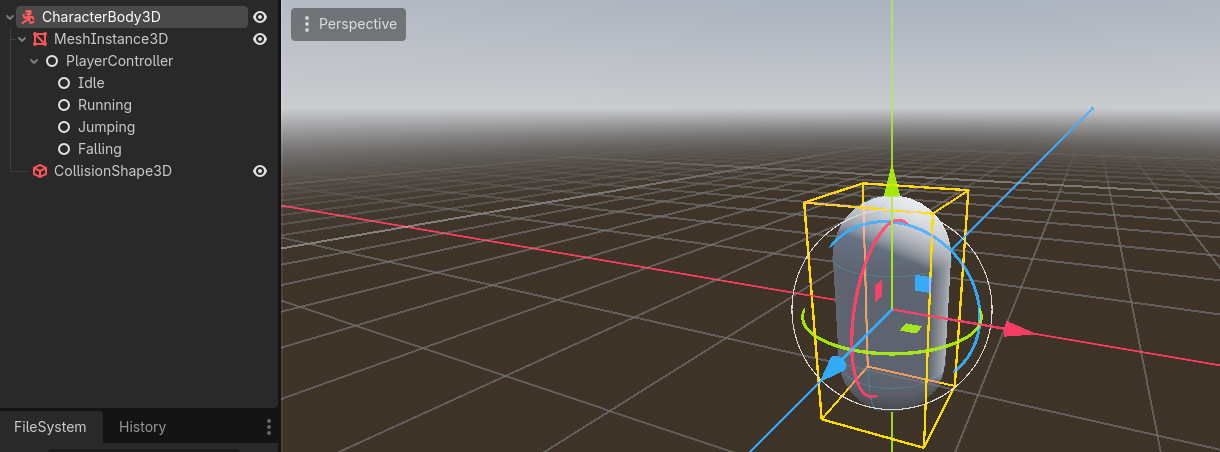
\includegraphics[width=\linewidth]{Images/BasePlayerScene.png}
	\caption{Képernyőkép a kezdetleges játékos színtérről}
	\label{BasicPlayerScene}
\end{figure}

Ahhoz, hogy a mozgásrendszert implementálni tudjam először el kellett gondolkoznom azon, hogy milyen más Node-ok fognak még esetleg kelleni nekem. Egyből tudtam, hogy kelleni fog egy kamera, ami a játékost követi, hogy láthassa a felhasználó, hogy mit is csinál. Továbbá, mint az a legtöbb játékban már megszokott és szinte elvárt, hogy a kamera kihasson a mozgás irányára. Így kibővítettem még három Node3D objektummal:
\begin{itemize}
	\item \textbf{CamRoot:} A kamera csoport gyökere, nincs kihatással a többi részre, csak csoportosítás szempontjából van használva.
	\item \textbf{CamYaw:} A kamera oldalirányú elmozdulásának nyílvántartásáért felel.
	\item \textbf{CamPitch:} A kamera magassági elmozdulásának nyílvántartásáért felel.
\end{itemize} 

A Node3D objektumok valójában pontok a háromdimenziós térben, így tökéletesen megfelelnek a különböző irányok nyílvántartására, ezért választottam inkább ezt a megoldást, mint azt, hogy változókat hozzak létre ezek figyelésére. 

Létrehoztam továbbá még egy SpringArm3D és egy Camera3D Node-ot is.

\begin{itemize}
	\item \textbf{SpringArm3D:} Ahogyan azt a nevéből is ki lehet venni, ez egy ún. "rugós kar", amely arra szolgál, hogy ha ütközik valamilyen akadállyal a színtérben, akkor mint egy rúgó elkezd összenyomódni. Ez arra kellett, hogy ha a kamera, ami ennek egy  gyermeke, esetleg belemenne a falba, akkor ne okozzon bajt.
	\item \textbf{Camera3D:} Ez a Node maga a kamera. Kivetít akármit amit a legközelebbi nézőtérből (viewport) lát, a fát felfelé bejárva. Ha nincs nézőtér a fában, akkor a globális nézőteret fogja használni.
\end{itemize}

Annak érdekében, hogy az állapotok könnyen nyomonkövethetőek legyenek csináltam egy pár CheckBox és Label Node-okból álló Control csoportot. A Control csoportok a Godot-on belül kétdimenziós síkok, amiket általában felhasználói felületnek szoktak használni. Ezt a csoportot a CamRoot alá rendeltem, így követni fogja a kamerát, ami annyit fog eredményezni, hogy a felhasználó képernyőjén folyamatosan láthatóak lesznek az elemek. Így egyenlőre a színtér az alábbi képen láthatóan néze ki[\ref{PlayerSceneComplete}].

\begin{figure}[H]
	\centering
	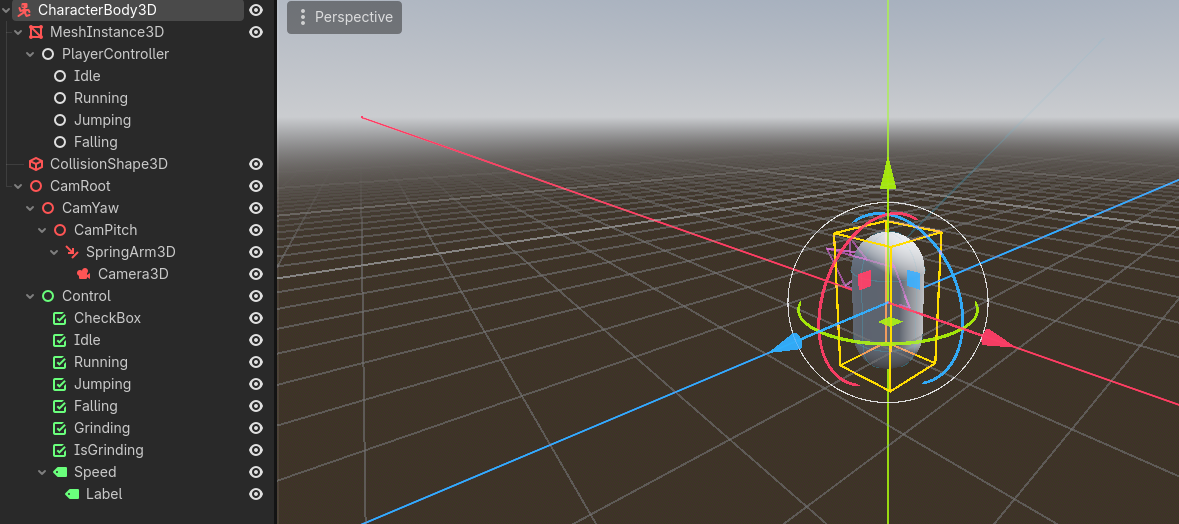
\includegraphics[width=\linewidth]{Images/PlayerSceneComplete.png}
	\caption{A befejezett játékos színtere}
	\label{PlayerSceneComplete}
\end{figure}

\subsection{Változtatások az állapotgéphez}

Ahogyan azt már a \hyperref[chap:FSM]{\ref{chap:FSM}. fejezet}, \hyperref[subsec:Prog]{\ref{subsec:Prog}. bekezdésében} is megadtam az automatánk két része a State és StateMachine osztályok nem változnak sokat.\\

A State osztályon belül:
\begin{itemize}
	\item Hozzáadtam egy "TransitionEventHandler" signal-t (jelzőt), amellyel az állapotok közötti változást tudom szabályozni.
	\item A "StateMachine" osztályt átneveztem "PlayerController"-re.
	\item Hozzáadtam egy "gravity" változót, amelyet, akármelyik állapot el tud érni, ha szüksége lenne rá.
	\item Hozzáadtam egy "movementDirection" nevű változót, amely egy három\-dimenziós vektor alakjában tárolja a felhasználói inputból kiszámított mozgási irányt.
\end{itemize}

Valamint az átnevezett PlayerController osztályon belül:
\begin{itemize}
	\item Hozzáadtam egy "TransitionToEventHandler" nevű signal-t, ami a külön\-bőző állapotok közötti átmenetért felel.
	\item Hozzáadtam egy Control és egy új Dictionary osztályú objektumot, amik vizuális debug-olásért lettek létrehozva. Miután összegyűjtöttük az összes CheckBox Node-ot, amik kellettek a legelsőt már aktiváljuk is. Az "OnTransitionTo" metóduson belül állítjuk a jelenleg megjelenített állapotot.
	\item Az "OnSetMovementState"" a jelenlegi mozgásállapotot állítja és az "OnSetMovementDirection" frissíti a jelenlegi állapot movementDirection változóját.
\end{itemize}

A PlayerController script-et hozzácsatoltam a megosztozó nevű PlayerController Node-ra a játékos színterén belül. A State osztály meghagyjuk magát nem csatoltam hozzá semmihez, ezt csak arra használtam, hogy az állapotokat ebből az osztályból tudjam leszármaztatni.

\subsection{Az állapotok megvalósítása}

Ha visszaemlékeznek, a \hyperref[chap:Concept]{\ref{chap:Concept}. fejezet}, \hyperref[subsec:States]{\ref{subsec:States}. alszakaszában} vázoltam az állapotgé\-pet és a különböző tervezett állapotokat és az azok közötti átmenetet. Most ezek megvalósításáról szeretnék beszélni.
Mindegyik állapot implementációját röviden át fogom beszélni és a fontosabbakat ki fogom emelni és bele fogok menni a matekba is háttérben. A kódot nem minden esetben fogom ide beírni, viszont a CD mellékletben megtalálják a forráskódot, valamint a \hyperref[cover:UseCase]{\ref{cover:UseCase}CD Használati útmutató oldalon} elmondottak alapján tudják követni részletesebben a kódot.\\

A megvalósítás során az állapotokat egy időben írtam a játékos script-jével. Létrehoztam egy Player scriptet és osztályt, amit a CharacterBody3D Node-hoz csatoltam. Ezen az osztályon belül hoztam létre azokat a metódusokat, amelyeket az állpotátmenetek vizsgálására használtam. Valamint itt számítottam ki a kamera mutatási irányát és a mozgásvektort is.\\

Az állapotok implementáció sorrendjében:
\begin{itemize}
	\item \textbf{Idle:} Az Idle állapot azért felelős, hogy a mozgást megállítsa. Ha a játékos már mozgásban volt, akkor a beépített "MoveToward" metódus segítségével csökkenti a sebességét nullára. Ahhoz, hogy a játékos ide eljusson egy beépített metódust segítségével az "IsOnFloor"-ral megnézem, hogy a karakter a földön tartózkodik-e és, hogy e közben nincs-e letartva semelyik mozgás gomb.\\
	\item \textbf{Running:} A mozgás (vagy futás) állapotnál a játékos sebességét befolyásoljuk a movementDirection attribútummal, ami megadj egy mozgás vektort. Ezt a vektort a "Player" osztályon belül számítjuk ki
\end{itemize}


